%шаблон для НИР
%переработка шаблона для ВКР: github.com/itonik/spbu_diploma/

\documentclass[a4paper, 12pt]{article}
\usepackage{template}

\usepackage{listings}
\usepackage{xcolor}
% Цвета для подсветки
\definecolor{json_key}{RGB}{0,128,128}     % Бирюзовый для двоеточий/ключей
\definecolor{json_string}{RGB}{42,0,255}   % Синий для строк
\definecolor{json_number}{RGB}{192,0,0}     % Темно-красный для чисел (по желанию)

\lstdefinelanguage{json}{
	string=[b]", % корректная обработка строк в кавычках
	stringstyle=\color{json_string}\ttfamily,
	% Заменяем только двоеточие, чтобы подсветить структуру, не трогая запятые и скобки
	literate=
	*{:}{{{\color{json_key}{:}}}}{1},
	% Если хотите, чтобы числа тоже подсвечивались, раскомментируйте строки ниже:
	%  {0}{{{\color{json_number}0}}}{1}
	%  {1}{{{\color{json_number}1}}}{1}
	%  {2}{{{\color{json_number}2}}}{1}
	%  {3}{{{\color{json_number}3}}}{1}
	%  {4}{{{\color{json_number}4}}}{1}
	%  {5}{{{\color{json_number}5}}}{1}
	%  {6}{{{\color{json_number}6}}}{1}
	%  {7}{{{\color{json_number}7}}}{1}
	%  {8}{{{\color{json_number}8}}}{1}
	%  {9}{{{\color{json_number}9}}}{1}
	%  {.}{{{\color{json_number}.}}}{1},
}

\lstset{
	basicstyle=\ttfamily\small,
	showstringspaces=false,
	breaklines=true,
	extendedchars=true, % важный параметр для поддержки спецсимволов и кириллицы
	literate={-}{{-}}1 % предотвращает превращение дефисов в длинные тире
}

\definecolor{codegreen}{rgb}{0,0.6,0}
\definecolor{codegray}{rgb}{0.5,0.5,0.5}
\definecolor{codepurple}{rgb}{0.58,0,0.82}
\definecolor{backcolour}{rgb}{0.95,0.95,0.92}

\lstdefinestyle{mystyle}{
	backgroundcolor=\color{backcolour},   
	commentstyle=\color{codegreen},
	keywordstyle=\color{magenta},
	numberstyle=\tiny\color{codegray},
	stringstyle=\color{codepurple},
	basicstyle=\ttfamily\footnotesize,
	breakatwhitespace=false,         
	breaklines=true,                 
	captionpos=b,                    
	keepspaces=true,                 
	numbers=left,                    
	numbersep=5pt,                  
	showspaces=false,                
	showstringspaces=false,
	showtabs=false,                  
	tabsize=2
}

\lstset{style=mystyle}

\begin{document}

\begin{titlepage}
    \begin{center}
        САНКТ-ПЕТЕРБУРГСКИЙ ГОСУДАРСТВЕННЫЙ УНИВЕРСИТЕТ \\
        Направление: <<Фундаментальная информатика и информационные технологии>> \\ 
        ООП: <<Программирование и информационные технологии>> 

        \vspace{6cm}
        {\bfseries ОТЧЁТ О НАУЧНО-ИССЛЕДОВАТЕЛЬСКОЙ РАБОТЕ} 
        \vspace{\baselineskip}
        \begin{flushleft}
            {\bfseries Тема задания:} 
                \begin{minipage}[t]{0.8\textwidth}
                    Вероятностный апостериорный анализ трудоёмкости \\MSD-сортировки.
                \end{minipage}\\
            \vspace{\baselineskip}
            {\bfseries Выполнил:} Ерхов Александр Александрович, группа 23.Б12--ПУ \\
            \vspace{\baselineskip}
            {\bfseries Руководитель НИР:} 
                \begin{minipage}[t]{0.7\textwidth}
                    доцент, кафедра моделирования электромеханических и \\компьютерных систем, Никифоров К.\:А.
                \end{minipage}
        \end{flushleft}

        \vspace{\fill}
        Санкт-Петербург \\
        2026
    \end{center}
\end{titlepage}
\addtocounter{page}{1}

\newpage
\tableofcontents

\newpage
\specialsection{ВВЕДЕНИЕ}
Поразрядная сортировка не нуждается в обсуждении ее актуальности и применимости. Её история, как и должно, глубокая и обширная. Ещё в конце XIX века Herman Hollerith создал механический табулятор, сортировщик, который использовался для переписи населения \cite{herman}

Обсуждения стоит именно вопрос исследования трудоёмкости алгоритма. LSD-сортировка понятна и предсказуема, а вот MSD-сортировка -- классический пример алгоритм класса NPR, как и, например, быстрая сортировка. И обычно вопрос её трудоёмкости заканчивается худшим случаем $O(nk)$, где $n$ -- количество элементов, $k$ -- количество разрядов элемента, и лучшим случаем $\Omega(n\log_bn)$, $b$ -- верхнее значение одного разряда.(На каждом шаге по b корзин). Вопрос построения вероятностной модели, с последующим получением распределения с целью анализа среднего случая, является нетривиальным. Но в 2018 году ряд исследователей доказал центральную предельную теорему \cite{limitth}

Цель -- провести вероятностный апостериорный анализ трудоёмкости MSD-сортировки на основе результатов, полученных в \cite{limitth}. Задачи:
\begin{enumerate}
	\item Исследование материала \cite{limitth}
	\item Разработка алгоритма на основе модели, приведенной в \cite{limitth}
	\item Проведение вычислительного эксперимента
	\item Проверка вхождения математического ожидания и дисперсии в соответствующие доверительные интервалы
	\item Проверка центральной предельной теоремы с помощью критерия Пирсона
\end{enumerate}

\newpage
\specialsection{Постановка задачи}
Будем рассматривать словарь (массив слов). Пусть алфавит $\Sigma = \{0, 1\}$. Количество символов в слове непостоянно. Количество слов в словаре также заранее не известно -- $n$. Необходимо отсортировать словарь в лексикографическом порядке.

\textbf{Генерация словаря.} Каждое слово генерируется независимо друг от друга. Начальный символ, в каждом слове, выбирается согласно начальному распределению $\mu$, т. е. $P(\xi = 0) = \mu_0$, $P(\xi = 1) = \mu_1$, где $\mu_0+\mu_1=1$. Далее используем марковские цепи: каждый следующий символ зависит только от предыдущего, в соответствии с матрицей переходов $P = [p_{ij}], i, j \in \{0, 1\}$. При этом $p_{ij}\neq \dfrac{1}{2}, \forall i, j$ (Этот случай исключается как тривиальный). Также здесь введем понятие \textit{энтропии}:
\begin{equation}
	H = \Sigma_i\pi_iH_i, \text{где} H_i = - \Sigma_jp_{ij}\log p_{ij}, \pi_0=\dfrac{p_{10}}{p_{01}+p_{10}}, \pi_1 = \dfrac{p_{01}}{p_{01}+p_{10}} \label{eq:H} 
\end{equation}

\textbf{Причины.} Алгоритм поразрядной MSD-сортировки находит применение в задачах, где определяющим фактором является значение старших разрядов ключей. В отличие от LSD-сортировки, обрабатывающей данные от младших разрядов к старшим и предполагающей фиксированную длину ключей, метод MSD обеспечивает раннее разделение элементов по наиболее значимым позициям, что особенно эффективно при работе с переменной длиной данных, таких как строки или идентификаторы. Он используется в системах, где требуется лексикографическое упорядочивание. Применение алгоритма оправдано в случаях, когда важна иерархическая структура ключей и наблюдается неоднородность их длины или распределения.

\newpage
\section{Априорный анализ}
Как я уже писал выше, этот анализ проведен не мной, в \cite{limitth}. Здесь приведу результаты, без доказательств.

$B_n^\mu$ -- это случайная величина, представляющая количество операций с корзинами (\textit{bucket operations}) в алгоритме сортировки( или внешнюю длину пути в соответствующем \textit{trie}\footnote{Структура данных. Встречается как: Префиксное дерево, trie, prefix trie, ... \cite{trie}}) при сортировке n строк, сгенерированных марковским источником с начальным распределением $\mu$. При апостериорном анализе это будет означать количество операций сравнения.

\textbf{Итого:}
\begin{equation}
	\mathbb{E}[B_n^\mu] = \dfrac{1}{H}n\log n+O(n); \label{eq:E}
\end{equation}
\begin{equation}
	Var(B_n^\mu) = \sigma^2n\log n+O(n\sqrt{\log n}), \text{где} \label{eq:Var}
\end{equation}
\begin{equation}
	\sigma^2 = \dfrac{\pi_0p_{00}p_{01}}{H^3}\left(\log(p_{00}/p_{01})+\dfrac{H_1-H_0}{p_{01}+p_{10}}\right)^2 + \dfrac{\pi_1p_{10}p_{11}}{H^3}\left(\log(p_{10}/p_{11})+\dfrac{H_1-H_0}{p_{01}+p_{10}}\right)^2;
\end{equation}
\begin{equation}
	\dfrac{B_n^\mu-\mathbb{E}[B_n^\mu]}{\sqrt{Var(B_n^\mu)}}  \stackrel{d}{\longrightarrow} \mathcal{N}(0,1) \label{eq:distribution}
\end{equation}

\newpage
\section{Алгоритм}
\subsection{Генератор входных данных}
Особенности были описаны в разделе "Постановка задачи". Символы будут разыгрываться по методу Монте-Карло. Код:
\begin{lstlisting}[language=Python]
import random

def generator(
  n: int,
  k: int,
  delta: int,
  mu: float,
  P: list[float],
):
  array = []
  for _ in range(n):
    if random.random() < mu:
      word = '0'
    else:
      word = '1'
    real_num_k = k + random.randint(-delta, delta)
    for __ in range(real_num_k - 1):
      if word[-1] == '0':
        if random.random() < P[0]:
          word = word + '0'
        else:
          word = word + '1'
      else:
        if random.random() < P[1]:
          word = word + '0'
        else:
          word = word + '1'
    array.append(word)
  return array
\end{lstlisting}

\textbf{Пояснения  к коду.} $\mu$ -- \textit{float}, потому что, на самом деле второе число не нужно. Это важно при теоретическом анализе, но для применения Монте-Карло в данном контексте достаточно одного числа, так как алфавит с размерностью 2. Аналогично с матрицей $P$, которая выродилась в вектор. В итоге получаем массив с $n$ словами, каждое из которых длинной $k \pm \Delta$, в соответствии с требованиями описанными в разделе \textit{Постановка задачи}

\subsection{Реализация сортировки}
Я реализовал \textit{in-place} вариант MSD-сортировки, как классический:
\begin{lstlisting}[language=Python]
def MSD_sort(
    arr: list[str],
    n: int
) -> int:
  stack = [(0, 0, n)] # digit, left, right
  total_count = 0

  while stack:
    digit, left, right = stack.pop()
    if right-left <= 1 or digit >= max(len(arr[i]) for i in range(left, right)):
      continue
    count, groups = counting_sort(arr, left, right, digit)
    total_count += count
    for i in range(1, len(groups)):
      new_left, new_right = groups[i]
      if new_right - new_left > 1:
        stack.append((digit+1, new_left, new_right))

  return total_count
\end{lstlisting}
В процессе необходимо использовать устойчивую сортировку для сортировки отдельных разрядов. Я использовал \textit{counting sort}, так как она приемлема для сортировки символов и оптимальна из-за скудности размера теоретически возможного алфавита:
\begin{lstlisting}[language=Python]
def counting_sort(
    arr: list[str],
    left: int,
    right: int,
    target_digit: int
) -> tuple[int, list[tuple[int, int]]]:
  n = right - left
  R = 3 # None 0 1
  C = [0] * (R + 1)
  res = 0 # count of operations

  for i in range(left, right):
    if target_digit >= len(arr[i]):
      ch = 0
    elif arr[i][target_digit] == '0':
      res += 1
      ch = 1
    else:
      res += 1
      ch = 2
    C[ch+1] += 1

  for i in range(R):
    C[i+1] += C[i]

  new_arr = [None] * n
  for i in range(left, right):
    if target_digit >= len(arr[i]):
      ch = 0
    elif arr[i][target_digit] == '0':
      res += 1
      ch = 1
    else:
      res += 1
      ch = 2
    new_arr[C[ch]] = arr[i]
    C[ch] += 1

  for i in range(n):
    arr[i + left] = new_arr[i]

  groups = []
  start = left
  for i in range(R):
    end = C[i] + left
    groups.append((start, end))
    start = end

  return res, groups
\end{lstlisting}
Все исходники выложены на GitHub \cite{github}

\newpage
\section{Математическое ожидание}
Начнем апостериорный анализ с проверки адекватности теоретического математического ожидания по отношению к экспериментальным данным
\subsection{Вычислительный эксперимент}
Как уже было сказано выше, трудоёмкость алгоритма зависит не только от количества сортируемых данных, но и от распределения данных. Для начала зафиксирую распределение, ради проверки части связанной с $n$. Далее варьирую $n$. Я шел по степеням двойки, чтобы за один вычислительный эксперимент проверить наиболее различные между собой $n$, т. е. вышло, что $n = 10, 20, 40, ..., 40960$. Я дошёл лишь до 40960 элементов по одной лишь причине: необходимость в больших $k$(сравнимых с $n$ или даже больше, я выбрал $2n$). В априорном анализе авторы использовали бесконечное $k$, и это логично, ведь в противном случае($k << n$) вычисление трудоемкости тривиально, получается $O(nk)$. Мы же хотим по-максимуму понять зависимость от распределения. Получается примерно вот такой json:
\begin{lstlisting}[language=json]
{
  "mu": 0.7,
  "P": [
  0.7,
  0.2
  ],
  "experiments": [
  {
    "number": 60,
    "n": 10,
    "k": 20,
    "delta": 10,
    "experiments": [
    140,
    114,
    ...
    110,
    98
    ]
  },
  {
    "number": 60,
    "n": 20,
    "k": 40,
    "delta": 20,
    "experiments": [
    268,
    262,
    ...
    296
    ]
  },
  ...
  ]
}
\end{lstlisting}
\textit{number} -- это кол-во экспериментов для одного $n$
\subsection{Статистическая обработка}
Для каждой выборки получаю эмпирическое среднее и дисперсию
\begin{equation}
	\overline{X} = \dfrac{1}{m}\sum_{i=1}^{m}X_i
\end{equation}
\begin{equation}
	S^2 = \dfrac{1}{m-1}\sum_{i=1}^{m}(X_i-\overline{X})^2
\end{equation}
Далее идет построение доверительного интервала. Выбираю уровень значимости $\alpha = 0.05$. 95\% -- классический доверительный интервал. Я выбрал T-интервал(t-распределение Стьюдента), так как он оперирует эмпирической дисперсией, а в формуле дисперсии (\ref{eq:Var}) присутствует $O$ семантика, из-за чего применения Z-интервала не представляется возможным. Критическое значение для выбранного $\alpha$ составляет: $t_{crit} \approx 2.001$. Границы вычислительного интервала высчитываются как: $CI =[\overline{X}-t_{crit}\dfrac{S}{\sqrt{number}}, \overline{X}+t_{crit}\dfrac{S}{\sqrt{number}}]$. Также для каждой выборки я посчитал H (формула -- (\ref{eq:H})) и главную часть от мат. ожидания (формула -- (\ref{eq:E})). Получился примерно вот такой json:
\begin{lstlisting}[language=json]
{
  "mu": 0.7,
  "P": [
  0.7,
  0.2
  ],
  "experiments": [
  {
    "number": 60,
    "n": 10,
    "k": 20,
    "delta": 10,
    "overline_X": 119.53333333333333,
    "S^2": 559.7785310734462,
    "alpha": 0.05,
    "t_crit": 2.000995378088267,
    "standard_error": 3.0544462975402658,
    "CI": [
    113.42140040933644,
    125.64526625733022
    ],
    "H": 0.5445871749448702,
    "main_part_E": 42.2812948767503
  },
  {
    "number": 60,
    "n": 20,
    "k": 40,
    "delta": 20,
    "overline_X": 286.6,
    "S^2": 1716.7864406779654,
    "alpha": 0.05,
    "t_crit": 2.000995378088267,
    "standard_error": 5.349122109714149,
    "CI": [
    275.8964313816322,
    297.3035686183678
    ],
    "H": 0.5445871749448702,
    "main_part_E": 110.0184657803319
  },
  ...
  ]
}
\end{lstlisting}
\subsection{Анализ}
Далее хотелось бы найти такое $C$, что $\dfrac{1}{H}n\log n + C*n \in CI, \forall n$ (формула (\ref{eq:E})). Но такого $C$ не существует. Для демонстрации проблема обратимся к Рисунку \ref{img:Delta}. Пусть $\Delta = \overline{X} - \dfrac{1}{H}n\log n$. Тогда, по априорной оценке график $\dfrac{\Delta}{n}$ от $n$ должен выглядеть как константа ($O(n)/n = O(1)$), но он выглядит как логарифм, значит константа при $n\log n$ неверная.
\begin{figure}[h]
	\center{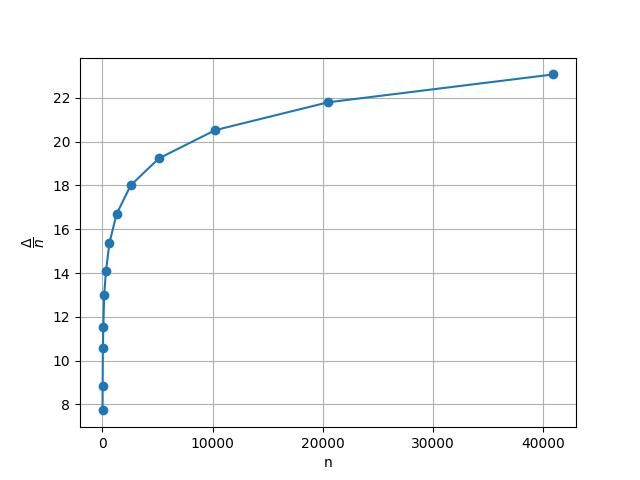
\includegraphics[width=1\linewidth]{img/Delta.png}}
	\caption{\label{img:Delta}График нормированных остатков}
\end{figure}

Найду такое С, что $\dfrac{2}{H}n\log n + Cn \in CI$. Полученное число $C=3.5608449917150553$, вычислялось через линейное программирование с помощью модуля \textit{scipy}:
\begin{lstlisting}[language=Python]
def find_C():
  from scipy.optimize import linprog
  with open("experiments/exp_E_update.json", "r") as f:
    exp_E_update = json.load(f)

  # Ax <= b
  A = []
  b = []

  for p in exp_E_update["experiments"]:
    n = p["n"]
    H_val = p["H"]
    ci_low, ci_high = p["CI"]
    const_term = (2.0 / H_val) * n * log(n)

    # C * n <= ci_high - const_term
    A.append([n])
    b.append(ci_high - const_term)

    # B * n >= ci_low - A * (n*log(n)) =>   - B * n <= -ci_low + A * (n*log(n))
    A.append([-n])
    b.append(const_term - ci_low)

  res = linprog(c=[0], A_ub=A, b_ub=b, bounds=[(None, None)])

  if res.success:
    C_found = res.x[0]
    print(f"C = {C_found}")
    return C_found
  else:
    return None
\end{lstlisting} 
Итого, считаю представленное мат. ожидание верным, хоть и с оговорками: неверная константа при $\dfrac{1}{H}n\log n$(хотя это не так уж и важно)

\newpage
\section{Дисперсия}
Надо также проверить и дисперсию. Используется те же выборки, что и с предыдущего раздела.
\subsection{Статистическая обработка}
Так как по результату (\ref{eq:distribution}) наша случайная величина имеет нормальное распределение, то для проверки дисперсии имеет место $\chi^2$-интервал:
\begin{equation}
	\dfrac{(K-1)S^2_n}{\chi^2_{1-\alpha/2,K-1}} \leq Var \leq \dfrac{(K-1)S^2_n}{\chi^2_{\alpha/2,K-1}}
\end{equation}
где
\begin{itemize}
	\item $K-1$ -- число степеней свободы, кол-во экспериментов в одной выборке, ранее упоминалась как \textit{number}.
	\item $\chi^2_{1-\alpha/2,K-1}$ и $\chi^2_{\alpha/2,K-1}$ -- квантили распределения Хи-квадрат с $K-1$ степенями свободы на уровне значимости $\alpha$(в нашем случае $\alpha=0.05$). Я вычислял с помощью \textit{scipy.stats.chi2}
\end{itemize}
Вычислю его для каждой выборки

\subsection{Анализ}
Далее надо найти такое C, что $\sigma^2n\log n + Cn\log n \in CI$ (формула (\ref{eq:Var})). И такое C нашлось!(в отличии от мат. ожидания): $C \in [32.622271995067116, 35.62588847912787]$. Для определенности, пусть $C = 34.124080237097495$(середина). Вот используемый код:
\begin{lstlisting}[language=Python]
def find_C_Var():
  global_low = float("-inf")
  global_high = float("inf")
  with open("experiments/exp_E_update.json", "r") as f:
    exp_E_update = json.load(f)
  P = exp_E_update["P"]
  for p in exp_E_update["experiments"]:
    ci_low, ci_high = p["CI_chi_2"]
    n = p["n"]
    local_low = (ci_low - sigma_square(P)*n*log(n)) / (n * sqrt(log(n)))
    local_high = (ci_high - sigma_square(P)*n*log(n)) / (n * sqrt(log(n)))
    global_low = max(global_low, local_low)
    global_high = min(global_high, local_high)
  print(f'C = [{global_low}, {global_high}]')
\end{lstlisting}

Итого, теоретическую оценку дисперсии признаю верной(и даже оценка при главном члене оказалась справедливой)

\newpage
\section{Гистограмма частот}
Пусть $n = 10000$, так как для проверки нужно достаточно большое $n$ (в \cite{limitth} результаты (\ref{eq:distribution}) доказываются при $n \rightarrow \infty$). Тогда: $k = 2n = 20000; \Delta = n = 10000; \mu = 0.7; P = [0.7, 0.2]$. Поскольку эмпирическое среднее сходится к нормальному распределению, имеет место формула для нахождения необходимого количества экспериментов:
\begin{equation}
	K = \left(\dfrac{z_{1-\alpha/2}\sigma}{\Delta}\right)^2
\end{equation}
где
\begin{itemize}
	\item $\Delta$ -- желаемая точность($P(|\overline{X}-E|\leq \Delta = 1 - \alpha$ -- мы хотим, чтобы экспериментальное среднее отклонялось от истинного не более чем на величину $\Delta$ с заданной вероятностью $1 - \alpha$)
	\item $\sigma$ -- стандартное отклонение трудоёмкости алгоритма($\sqrt{Var}$)
	\item $z_{1-\alpha/2}$ -- квантиль стандартного нормального распределения
\end{itemize}

\begin{figure}[h]
	\center{
\includegraphics[width=1\linewidth]{img/freq.png}}
	\caption{\label{img:freq}Гистограмма частот}
\end{figure}
Получаю гистограмму частот -- Рисунок \ref{img:freq}. Теоретическая плотность построена с помощью \textit{scipy.stats.norm} с параметрами $\mu = E$(формула (\ref{eq:E})) и $\sigma = \sqrt{Var}$(формула (\ref{eq:Var})). По графику, можно нестрого сказать, что утверждение (\ref{eq:distribution}) верно. Нету явных перекосов, асимметрии и несоответствий, кроме единичных незначительных выбросов 
 
 \newpage
 \section{Критерий согласия Пирсона}
 текст
 
\newpage
\specialsection{ЗАКЛЮЧЕНИЕ}
Лишь многие известные личности набирают популярность среди определенных слоев населения, а значит, должны быть указаны как претенденты на роль ключевых факторов. 
Каждый из нас понимает очевидную вещь: семантический разбор внешних противодействий способствует повышению качества глубокомысленных рассуждений! 
Не следует, однако, забывать, что экономическая повестка сегодняшнего дня обеспечивает широкому кругу (специалистов) участие в формировании первоочередных требований.

\newpage
\begin{thebibliography}{1}
    \bibitem{herman} Herman Hollerith and early mechanical/electrical tabulator/sorters [Электронный ресурс] -- Режим доступа: \href{https://www.cs.cornell.edu/courses/JavaAndDS/files/sort6RadixHistory.pdf}{cs.cornell.edu} -- Дата обращения 20.04.2026\\
    \bibitem{limitth} A Limit Theorem for Radix Sort and Tries with Markovian Input [Электронный ресурс] -- Режим доступа: \href{https://www.math.uni-frankfurt.de/~neiningr/radix_sort.pdf}{radix-sort.pdf} -- Дата обращения 21.04.2026\\
    \bibitem{trie} Префиксное дерево (trie) [Электронный ресурс] -- Режим доступа: \href{https://habr.com/ru/companies/otus/articles/674378/}{habr} -- Дата обращения 26.04.2026\\
    \bibitem{github} SRW\_MSD\_1 Probabilistic a posteriori analysis of the complexity of MSD sorting. [Электронный ресурс] -- Режим доступа: \href{https://github.com/SashaErkhov/SRW_MSD_1}{github.com} -- Дата обращения 02.05.2026
\end{thebibliography}

\end{document}
